\documentclass[]{elsarticle} %review=doublespace preprint=single 5p=2 column
%%% Begin My package additions %%%%%%%%%%%%%%%%%%%
\usepackage[hyphens]{url}

  \journal{Journal of Transport \& Health} % Sets Journal name


\usepackage{lineno} % add
\providecommand{\tightlist}{%
  \setlength{\itemsep}{0pt}\setlength{\parskip}{0pt}}

\usepackage{graphicx}
\usepackage{booktabs} % book-quality tables
%%%%%%%%%%%%%%%% end my additions to header

\usepackage[T1]{fontenc}
\usepackage{lmodern}
\usepackage{amssymb,amsmath}
\usepackage{ifxetex,ifluatex}
\usepackage{fixltx2e} % provides \textsubscript
% use upquote if available, for straight quotes in verbatim environments
\IfFileExists{upquote.sty}{\usepackage{upquote}}{}
\ifnum 0\ifxetex 1\fi\ifluatex 1\fi=0 % if pdftex
  \usepackage[utf8]{inputenc}
\else % if luatex or xelatex
  \usepackage{fontspec}
  \ifxetex
    \usepackage{xltxtra,xunicode}
  \fi
  \defaultfontfeatures{Mapping=tex-text,Scale=MatchLowercase}
  \newcommand{\euro}{€}
\fi
% use microtype if available
\IfFileExists{microtype.sty}{\usepackage{microtype}}{}
\bibliographystyle{elsarticle-harv}
\ifxetex
  \usepackage[setpagesize=false, % page size defined by xetex
              unicode=false, % unicode breaks when used with xetex
              xetex]{hyperref}
\else
  \usepackage[unicode=true]{hyperref}
\fi
\hypersetup{breaklinks=true,
            bookmarks=true,
            pdfauthor={},
            pdftitle={How do school travel planning stakeholders frame active school travel in Ontario, Canada?},
            colorlinks=false,
            urlcolor=blue,
            linkcolor=magenta,
            pdfborder={0 0 0}}
\urlstyle{same}  % don't use monospace font for urls

\setcounter{secnumdepth}{0}
% Pandoc toggle for numbering sections (defaults to be off)
\setcounter{secnumdepth}{0}

% Pandoc citation processing

% Pandoc header
\usepackage{booktabs}
\usepackage{longtable}
\usepackage{array}
\usepackage{multirow}
\usepackage{wrapfig}
\usepackage{float}
\usepackage{colortbl}
\usepackage{pdflscape}
\usepackage{tabu}
\usepackage{threeparttable}
\usepackage{threeparttablex}
\usepackage[normalem]{ulem}
\usepackage{makecell}
\usepackage{xcolor}



\begin{document}
\begin{frontmatter}

  \title{How do school travel planning stakeholders frame active school travel in
Ontario, Canada?}
    \author[Some Department]{Author 1\corref{1}}
   \ead{author1@example.com} 
    \author[Some Department]{Author 2}
   \ead{author2@example.com} 
    \author[Another University]{Author 3\corref{2}}
   \ead{author3@example.com} 
    \author[Some Institute]{Author 4\corref{2}}
   \ead{author4@example.com} 
    \author[Some University]{Author 5}
   \ead{author5@example.com} 
    \author[Some Department]{Author 6}
   \ead{author6@example.com} 
      \address[Some Department]{Department, Street, City, Province, Postal Code}
    \address[Another University]{Department, Street, City, Province, Postal Code}
    \address[Some Institute]{Street, City, Province, Postal Code}
    \address[Some University]{Department, Street, City, Province, Postal Code}
      \cortext[1]{Corresponding Author}
    \cortext[2]{Equal contribution}
  
  \begin{abstract}
  This is the abstract.
  
  It consists of two paragraphs.
  \end{abstract}
  
 \end{frontmatter}

\textbf{\emph{Background}}:\\
\textbf{\emph{Methods}}:\\
\textbf{\emph{Results}}: \textbf{\emph{Conclusions}}:

\newpage

\hypertarget{introduction}{%
\section{1. Introduction}\label{introduction}}

\hypertarget{school-travel-planning-in-canada}{%
\subsection{1.1. School travel planning in
Canada}\label{school-travel-planning-in-canada}}

Walking and bicycling to school, commonly known as active school travel
or active school transportation (AST), has been declining in Canada and
North America for decades ({\textbf{???}}), with levels much lower than
other developed countries like The Netherlands ({\textbf{???}}) and
Japan ({\textbf{???}}). This trend has prompted a multi-sector response
to identify strategies to increase AST, the most popular of which is a
growing interest in school travel planning across Canada.

School travel planning (STP) is a ``school-specific'' intervention led
by a facilitator that brings together a committee of stakeholders from
diverse sectors including education, planning, transportation, and
public health ({\textbf{???}}). Parents and parent councils also
typically have a role in supporting or implementing STP. The
intervention encourages participation from the broader community and
collaboration between involved stakeholders, who contribute their
expertise to remove ``school-specific'' barriers to AST and to identify
strategies for promoting and encouraging AST. STP may also involve other
stakeholders including local advocacy groups or environmental
organizations who are familiar with the state of AST at the
community-level. Buliung et al.~({\textbf{???}}) piloted an STP
intervention at 12 schools in 4 Canadian provinces and reported that it
increased AST rates and led to a ``mobilization of diverse community
resources''. Since this seminal study, STP interventions have become
increasingly popular and common at schools across Canada and have even
attracted funding from provincial governments.

\hypertarget{correlates-of-active-school-travel}{%
\subsection{1.2. Correlates of active school
travel}\label{correlates-of-active-school-travel}}

Factors that influence AST are typically conceptualized according to the
socioecological model whereby children's travel behaviour is understood
within the context of their household, social, and built environments
(see {\textbf{???}}). At the individual level, older child age is often
associated with AST ({\textbf{???}}; {\textbf{???}}; {\textbf{???}}).
There is some evidence that gender is a determinant of AST
({\textbf{???}}; {\textbf{???}}), although this is not a strong or
consistent finding ({\textbf{???}}; {\textbf{???}}). Distance between
home and school is associated with AST ({\textbf{???}}; {\textbf{???}};
{\textbf{???}}; {\textbf{???}}) with less AST reported among children
who have to travel farther to school. Car ownership is an important
household-level influence on AST ({\textbf{???}}; {\textbf{???}};
{\textbf{???}}), as is household income ({\textbf{???}}). Parental
perceptions of the environment ({\textbf{???}}; {\textbf{???}}) and
children's skills ({\textbf{???}}) also influence whether they allow
their children to walk or cycle to school. Finally, many studies have
found that the quality of the built environment ({\textbf{???}};
{\textbf{???}}) and active travel infrastructure ({\textbf{???}})
facilitate AST. Concerns about traffic and strangers have been reported
by parents who drive their children to school ({\textbf{???}}). The
consensus is that all of these factors are interrelated and that
interventions ought to target multiple factors in order to increase
walking and bicycling levels to school.

\hypertarget{benefits-of-ast}{%
\subsection{1.3. Benefits of AST}\label{benefits-of-ast}}

The desire to increase AST is warranted - there is strong evidence that
children who walk and bicycle to school accrue physical and mental
health benefits. Many studies and reviews have focused on the
association between AST or CIM and physical activity (e.g.,
{\textbf{???}}; {\textbf{???}}; {\textbf{???}}), with findings
consistently demonstrating that children who travel by walking or
bicycling to school are more active than their peers who do not use
active travel. More recently, researchers have been exploring the link
between transport and children's wellbeing ({\textbf{???}};
{\textbf{???}}), which has relevant applications to the study of school
travel and satisfaction (see {\textbf{???}}). CIM is also important for
different domains of children's health and wellbeing ({\textbf{???}}).
It offers benefits such as increasing traffic and safety skills,
boosting spatial awareness when navigating public spaces, and providing
more opportunity for social interaction with peers ({\textbf{???}}).

\hypertarget{encouraging-adoption-of-active-school-travel}{%
\subsection{1.4. Encouraging adoption of active school
travel}\label{encouraging-adoption-of-active-school-travel}}

To increase rates of walking and bicycling independently to school,
Riazi et al.~({\textbf{???}}) state: ``it will be vital for
interventions to target modifiable factors, including children's and
parents' perceptions of their social environment.'' Parents play the
important role of ``gatekeeper'' by either granting or restricting CIM
licenses, meaning whether children can travel alone ({\textbf{???}}).
For this reason, stakeholders involved in STP produce information
targeted for both children and parents, and aim to involve the broader
community in their efforts to increase the number of children walking
and bicycling to school..

However, the ways in which interventions like STP are framed to their
target audience can ultimately influence how they are received and
whether they result in behaviour change. The correlates of AST are
important knowledge for policymakers because they identify points of
intervention and potential benefits that ought to be communicated to the
public encourage adoption of AST and to build support for new planning
paradigms. What is less clear is how CIM plays into the consideration of
policymakers when they act on the objective of increasing AST.

Any goals for AST, and also CIM, ought to be clearly articulated and
reflected in transportation plans and policies to guide initiatives.
Presently, however, there has been no study to date that explores how
Canadian municipalities and schools frame and discuss AST with the
public. Content analysis is one method to analyze how particular issues
are framed to groups of people, for instance parents or educators who
might be inclined to support AST. It attempts to understand how
information presented from a ``communicator'' leads the ``receiver'' to
a desired response ({\textbf{???}}). In a recent paper ({\textbf{???}}),
framing analysis was applied to review municipal policies addressing
climate change in four western Canadian cities. Natural language
processing (NLP) was used for a similar purpose to examine content in
general plans from Californian cities ({\textbf{???}}). The way policy
issues are framed is important to understand because it plays a role in
either altering or preserving the existing social perceptions.

\hypertarget{study-aim}{%
\subsection{1.5. Study aim}\label{study-aim}}

In 2017, the provincial government of Ontario in Canada issued funding
to Green Communities Canada (GCC), a non-profit organization, to launch
the \emph{Ontario Active School Travel} (OAST) program. The program
provides funding for school and community-based initiatives and supports
stakeholders in municipalities across the province to implement STP and
other interventions aimed at increasing AST. As of 2021, OAST has funded
\emph{X} projects in Ontario. GCC continues has funded projects across
Ontario led by collaborative groups involving school boards, municipal
or regional governments, and regional transportation consortia. The
latter are dedicated transportation bodies that deliver efficient and
effective transportation services, which generally focus on providing
the school busing service to families in their associated region.

The aim of this paper is to analyze how AST is framed by STP
stakeholders in Ontario, Canada. We used topic modelling and qualitative
content analysis to examine how the benefits and barriers of AST are
presented to the public and which solutions for improving AST are
identified in local policy documents from Ontario municipalities and
school boards. We compared these documents to a selection of studies on
AST to explore the extent to which research findings have trickled down
to inform policy and planning for AST interventions.

\hypertarget{data}{%
\section{2. Data}\label{data}}

\hypertarget{data-retrieval}{%
\subsection{2.1. Data retrieval}\label{data-retrieval}}

\hypertarget{policy-documents}{%
\subsubsection{2.1.1. Policy documents}\label{policy-documents}}

We then assembled a collection of publicly available documents that were
sourced online from the main stakeholder groups involved in STP
initiatives in Ontario: i) English school boards; ii) municipal
government; and iii) transportation consortia. Non-profit organizations,
police services, and advocacy groups are other stakeholders who may play
a role in supporting AST and/or STP, but this study does not include any
documents from these groups because they are not consistently
participating in initiatives.

The search was guided first by a list of all English school boards
across Ontario. The websites of each school board were searched for
pages related to transportation or school travel. These pages were
manually downloaded. Next, we collected documents by searching municipal
government and transportation consortia websites. The latter were
identified based on geographic area (i.e., the municipalities and/or
transportation consortia who are in the same geographic area of each
school board). Pages related to active transportation or school travel
were manually downloaded. Webpages were included in the corpus if they
were easy to find. This primary criteria was important since our
analysis pertains to how such issues are framed to the public. Thus,
these pages ought to be easy to find, which we defined as requiring no
more than 2-4 separate links from the initial Google search.

The initial corpus of policy documents included 64 relevant webpages
(i.e., one page or more) from all main stakeholder groups. It is
important to note that school boards, municipalities, and transportation
consortia may or may not publish information about their involvement in
AST and STP efforts on their respective websites or in policy documents.
Search results are summarized in Table \ref{tab:policy-documents}.

\begin{table}

\caption{\label{tab:policy-documents}\label{tab:search-results}Search results from the main STP stakeholder groups.}
\centering
\resizebox{\linewidth}{!}{
\begin{tabular}[t]{>{}l|>{\raggedright\arraybackslash}p{30em}|>{}l}
\toprule
Stakeholder & Total & Included\\
\midrule
\cellcolor{gray!6}{\textbf{English school boards}} & \cellcolor{gray!6}{62} & \cellcolor{gray!6}{31}\\
\textbf{Municipalities or regions} & 62 & 25\\
\cellcolor{gray!6}{\textbf{Transportation consortia}} & \cellcolor{gray!6}{39} & \cellcolor{gray!6}{8}\\
\bottomrule
\end{tabular}}
\end{table}

\hypertarget{academic-papers}{%
\subsubsection{2.2.1. Academic papers}\label{academic-papers}}

\hypertarget{data-cleaning}{%
\subsection{2.2. Data cleaning}\label{data-cleaning}}

A multi-step process was conducted to ensure that the analysis captured
as much content as possible from both the policy documents (n = 64) and
academic papers (n = 233). To begin, the webpages, which were manually
downloaded in portable document format (PDF), were trimmed so that pages
that only consisted of tables, figures, or references were removed. Many
academic papers were in a two-column format, which is not ideal for
conversion to \texttt{txt}. We adapted a procedure
(https://stackoverflow.com/questions/42541849/extract-text-from-two-column-pdf-with-r)
to read the two-column PDF documents so that they would be converted
correctly. Four academic papers did not join sufficiently and were taken
out of the corpus due to the substantial time required to manually
correct their inconsistencies.

Next, we converted the trimmed PDF documents into \texttt{txt} files so
that they could be imported in \texttt{R} for topic modelling. We then
proceeded to a manual cleaning phase where we removed any remaining
tables, figures, references, headers/footings, and captions that could
not be trimmed. Manual corrections were also required for certain pages
in academic papers that remained in two-column format after the
conversion process. This typically occurred on pages that had a table or
figure which disrupted the text. Finally, we reviewed all of the
documents to remove hyphenation by line breaks and to keep hyphenated
words together on the same line. Any ligatures (e.g., combinations of
characters or letters that were not properly detected during the
conversion process) were fixed by inserting the unicode sequence of
character to replace the missing sequence of characters.

We also manually removed any extraneous material in the academic papers
that did not pertain to AST specifically. This included footnotes,
references, acknowledgments, and conflict of interest statements in the
academic papers. We removed all phone numbers, inserted links to other
webpages, personal names, and content not to specific to AST from the
policy documents that were retrieved from the websites of school boards,
municipalities, and transportation consortia.

In the final step before analysis, we removed all blank spaces,
punctuation, capitalization, and numbers. English stop words, which are
common words such as \emph{and} or \emph{the} as identified in a
predetermined list by Lewis et al.~({\textbf{???}}) and other frequent
terms in the documents like ``school'' and location names were removed
from the corpora.

\hypertarget{methods}{%
\section{3. Methods}\label{methods}}

\hypertarget{natural-language-processing}{%
\subsection{3.1. Natural language
processing}\label{natural-language-processing}}

Natural language processing

Silge and Robinson ({\textbf{???}}) is

We've been using the unnest\_tokens function to tokenize by word, or
sometimes by sentence, which is useful for the kinds of sentiment and
frequency analyses we've been doing so far. But we can also use the
function to tokenize into consecutive sequences of words, called
n-grams. By seeing how often word X is followed by word Y, we can then
build a model of the relationships between them.

We do this by adding the token = ``ngrams'' option to unnest\_tokens(),
and setting n to the number of words we wish to capture in each n-gram.
When we set n to 2, we are examining pairs of two consecutive words,
often called ``bigrams'':

\hypertarget{content-analysis}{%
\subsection{3.2. Content analysis}\label{content-analysis}}

Content analysis is a method to examine content from texts including the
message itself, the sender(s) of the message, the recipients of the
message, or the impact of the message ({\textbf{???}}). Words or phrases
are the unit of analysis. \emph{Qualitative} content analysis

\hypertarget{reproducibility}{%
\subsection{3.3. Reproducibility}\label{reproducibility}}

This paper is an example of open and reproducible research that uses
only open software. All data were obtained from publicly available
sources and organized in the form of a data package. Following best
practices in spatial data science ({\textbf{???}}), the code and data
needed to reproduce or conduct a similar analysis for other regions in
North America or elsewhere are available for download.

\hypertarget{results}{%
\section{4. Results}\label{results}}

\hypertarget{word-and-document-frequency}{%
\subsection{4.1. Word and document
frequency}\label{word-and-document-frequency}}

We analyzed word and document frequency for each corpus. Table
\ref{tab:word-table} presents the most common terms found in the
municipal, transportation consortia, school board, and academic
documents.

\begin{table}

\caption{\label{tab:word-table}\label{tab:word-table}Top 25 terms identified in each corpora. Document frequencies are also indicated.}
\centering
\resizebox{\linewidth}{!}{
\begin{tabular}[t]{lcclcclcclcc}
\toprule
\multicolumn{3}{c}{Municipalities} & \multicolumn{3}{c}{School Boards} & \multicolumn{3}{c}{Transportation Consortia} & \multicolumn{3}{c}{Academic Papers} \\
\cmidrule(l{3pt}r{3pt}){1-3} \cmidrule(l{3pt}r{3pt}){4-6} \cmidrule(l{3pt}r{3pt}){7-9} \cmidrule(l{3pt}r{3pt}){10-12}
Term & Count (n) & Documents (n) & Term & Count (n) & Documents (n) & Term & Count (n) & Documents (n) & Term & Count (n) & Documents (n)\\
\midrule
\cellcolor{gray!6}{active} & \cellcolor{gray!6}{248} & \cellcolor{gray!6}{26} & \cellcolor{gray!6}{active} & \cellcolor{gray!6}{124} & \cellcolor{gray!6}{13} & \cellcolor{gray!6}{active} & \cellcolor{gray!6}{67} & \cellcolor{gray!6}{7} & \cellcolor{gray!6}{walking} & \cellcolor{gray!6}{5137} & \cellcolor{gray!6}{222}\\
travel & 126 & 20 & bus & 120 & 20 & walking & 55 & 8 & parents & 3946 & 211\\
\cellcolor{gray!6}{walking} & \cellcolor{gray!6}{90} & \cellcolor{gray!6}{25} & \cellcolor{gray!6}{students} & \cellcolor{gray!6}{119} & \cellcolor{gray!6}{30} & \cellcolor{gray!6}{walk} & \cellcolor{gray!6}{49} & \cellcolor{gray!6}{8} & \cellcolor{gray!6}{distance} & \cellcolor{gray!6}{3271} & \cellcolor{gray!6}{205}\\
bike & 87 & 15 & travel & 103 & 11 & travel & 41 & 8 & students & 2960 & 173\\
\cellcolor{gray!6}{cycling} & \cellcolor{gray!6}{78} & \cellcolor{gray!6}{22} & \cellcolor{gray!6}{student} & \cellcolor{gray!6}{93} & \cellcolor{gray!6}{25} & \cellcolor{gray!6}{students} & \cellcolor{gray!6}{39} & \cellcolor{gray!6}{9} & \cellcolor{gray!6}{cycling} & \cellcolor{gray!6}{2753} & \cellcolor{gray!6}{171}\\
\addlinespace
safety & 71 & 21 & information & 65 & 21 & safety & 32 & 6 & environment & 2631 & 202\\
\cellcolor{gray!6}{health} & \cellcolor{gray!6}{65} & \cellcolor{gray!6}{21} & \cellcolor{gray!6}{schools} & \cellcolor{gray!6}{61} & \cellcolor{gray!6}{19} & \cellcolor{gray!6}{help} & \cellcolor{gray!6}{29} & \cellcolor{gray!6}{9} & \cellcolor{gray!6}{activity} & \cellcolor{gray!6}{2371} & \cellcolor{gray!6}{209}\\
physical & 63 & 18 & board & 61 & 26 & schools & 25 & 9 & traffic & 2353 & 208\\
\cellcolor{gray!6}{traffic} & \cellcolor{gray!6}{59} & \cellcolor{gray!6}{20} & \cellcolor{gray!6}{walking} & \cellcolor{gray!6}{57} & \cellcolor{gray!6}{17} & \cellcolor{gray!6}{children} & \cellcolor{gray!6}{25} & \cellcolor{gray!6}{6} & \cellcolor{gray!6}{choice} & \cellcolor{gray!6}{2299} & \cellcolor{gray!6}{169}\\
road & 56 & 13 & walk & 53 & 13 & community & 24 & 7 & physical & 2256 & 215\\
\addlinespace
\cellcolor{gray!6}{activity} & \cellcolor{gray!6}{55} & \cellcolor{gray!6}{14} & \cellcolor{gray!6}{district} & \cellcolor{gray!6}{50} & \cellcolor{gray!6}{23} & \cellcolor{gray!6}{bus} & \cellcolor{gray!6}{18} & \cellcolor{gray!6}{4} & \cellcolor{gray!6}{trips} & \cellcolor{gray!6}{2194} & \cellcolor{gray!6}{170}\\
schools & 52 & 14 & weather & 40 & 11 & route & 17 & 5 & car & 2148 & 195\\
\cellcolor{gray!6}{children} & \cellcolor{gray!6}{47} & \cellcolor{gray!6}{15} & \cellcolor{gray!6}{safety} & \cellcolor{gray!6}{40} & \cellcolor{gray!6}{19} & \cellcolor{gray!6}{zone} & \cellcolor{gray!6}{16} & \cellcolor{gray!6}{6} & \cellcolor{gray!6}{safety} & \cellcolor{gray!6}{2140} & \cellcolor{gray!6}{204}\\
plan & 45 & 16 & safe & 39 & 19 & resources & 16 & 6 & time & 2101 & 218\\
\cellcolor{gray!6}{students} & \cellcolor{gray!6}{44} & \cellcolor{gray!6}{14} & \cellcolor{gray!6}{services} & \cellcolor{gray!6}{37} & \cellcolor{gray!6}{17} & \cellcolor{gray!6}{day} & \cellcolor{gray!6}{16} & \cellcolor{gray!6}{4} & \cellcolor{gray!6}{factors} & \cellcolor{gray!6}{2101} & \cellcolor{gray!6}{216}\\
\addlinespace
walk & 43 & 18 & planning & 37 & 7 & safe & 15 & 5 & child & 2085 & 187\\
\cellcolor{gray!6}{public} & \cellcolor{gray!6}{39} & \cellcolor{gray!6}{15} & \cellcolor{gray!6}{parents} & \cellcolor{gray!6}{32} & \cellcolor{gray!6}{17} & \cellcolor{gray!6}{planning} & \cellcolor{gray!6}{15} & \cellcolor{gray!6}{4} & \cellcolor{gray!6}{walk} & \cellcolor{gray!6}{2008} & \cellcolor{gray!6}{200}\\
will & 38 & 15 & sustainable & 31 & 8 & physical & 15 & 7 & public & 1983 & 208\\
\cellcolor{gray!6}{community} & \cellcolor{gray!6}{37} & \cellcolor{gray!6}{19} & \cellcolor{gray!6}{may} & \cellcolor{gray!6}{30} & \cellcolor{gray!6}{13} & \cellcolor{gray!6}{healthy} & \cellcolor{gray!6}{14} & \cellcolor{gray!6}{6} & \cellcolor{gray!6}{age} & \cellcolor{gray!6}{1783} & \cellcolor{gray!6}{211}\\
safe & 34 & 16 & children & 30 & 14 & traffic & 13 & 6 & urban & 1768 & 200\\
\addlinespace
\cellcolor{gray!6}{benefits} & \cellcolor{gray!6}{32} & \cellcolor{gray!6}{17} & \cellcolor{gray!6}{day} & \cellcolor{gray!6}{29} & \cellcolor{gray!6}{13} & \cellcolor{gray!6}{support} & \cellcolor{gray!6}{13} & \cellcolor{gray!6}{6} & \cellcolor{gray!6}{home} & \cellcolor{gray!6}{1715} & \cellcolor{gray!6}{199}\\
play & 31 & 2 & child & 29 & 12 & families & 13 & 5 & social & 1713 & 191\\
\cellcolor{gray!6}{resources} & \cellcolor{gray!6}{30} & \cellcolor{gray!6}{13} & \cellcolor{gray!6}{cancellations} & \cellcolor{gray!6}{29} & \cellcolor{gray!6}{13} & \cellcolor{gray!6}{way} & \cellcolor{gray!6}{12} & \cellcolor{gray!6}{5} & \cellcolor{gray!6}{different} & \cellcolor{gray!6}{1713} & \cellcolor{gray!6}{215}\\
healthy & 29 & 16 & routes & 28 & 14 & student & 12 & 5 & mobility & 1659 & 138\\
\cellcolor{gray!6}{routes} & \cellcolor{gray!6}{27} & \cellcolor{gray!6}{13} & \cellcolor{gray!6}{physical} & \cellcolor{gray!6}{28} & \cellcolor{gray!6}{11} & \cellcolor{gray!6}{region} & \cellcolor{gray!6}{12} & \cellcolor{gray!6}{4} & \cellcolor{gray!6}{significant} & \cellcolor{gray!6}{1650} & \cellcolor{gray!6}{208}\\
\bottomrule
\multicolumn{12}{l}{\rule{0pt}{1em}\textit{Note: }}\\
\multicolumn{12}{l}{\rule{0pt}{1em} }\\
\multicolumn{12}{l}{\rule{0pt}{1em}\textsuperscript{a} Count (n) refers to the total number of times the term is found in the corpora}\\
\multicolumn{12}{l}{\rule{0pt}{1em}\textsuperscript{b} Documents (n) refers to the total number of documents that feature the term}\\
\end{tabular}}
\end{table}

\hypertarget{bigrams-and-correlations}{%
\subsection{4.2. Bigrams and
correlations}\label{bigrams-and-correlations}}

Bigrams for each policy corpora are shown in Figures
\ref{fig:city-bigrams}, \ref{fig:consortia-bigrams}, and
\ref{fig:school-bigrams}. These figures help to make further sense of
the word frequencies reported above, and highlight the main ideas that
are presented to the public in each of the policy corpora.
Municipalities primarily discuss ``physical activity'' (n = 53) and
``public health'' (n = 19) in the context of active travel. In addition,
``travel planning'' (n = 19), ``bike lanes'' (n = 16), and ``safe
routes'' (n = 14) are also identified, conceivably as interventions and
built environment factors that support AST. Key issues related to AST
such as ``traffic safety'' (n = 10), ``air quality'' (n = 9), and
``greenhouse gases'' (n = 9) are conveyed to the public but in fewer
documents. Similar word bigrams are found in school board documents:
``travel planning'' (n = 33), ``safe routes'' (n = 15), ``physical
activity'' (n = 10), and ``public health'' (n = 10) are among the most
common bigrams. Unlike other STP stakeholders, school boards also
consider ``inclement weather'' (n = 24) ``bus cancellations'' (n = 13).
This is likely because many students in Ontario travel by school bus and
this information is presented alongside AST. Finally, transportation
consortia documents highlight ``physical activity'' (n = 10),
``pedestrian safety'' (n = 8), ``crossing guards'' (n = 6), ``travel
planning'' (n = 6), and ``walk zones'' (n = 6). Bicycling is notably
absent from transportation consortia documents.

\begin{figure}

{\centering 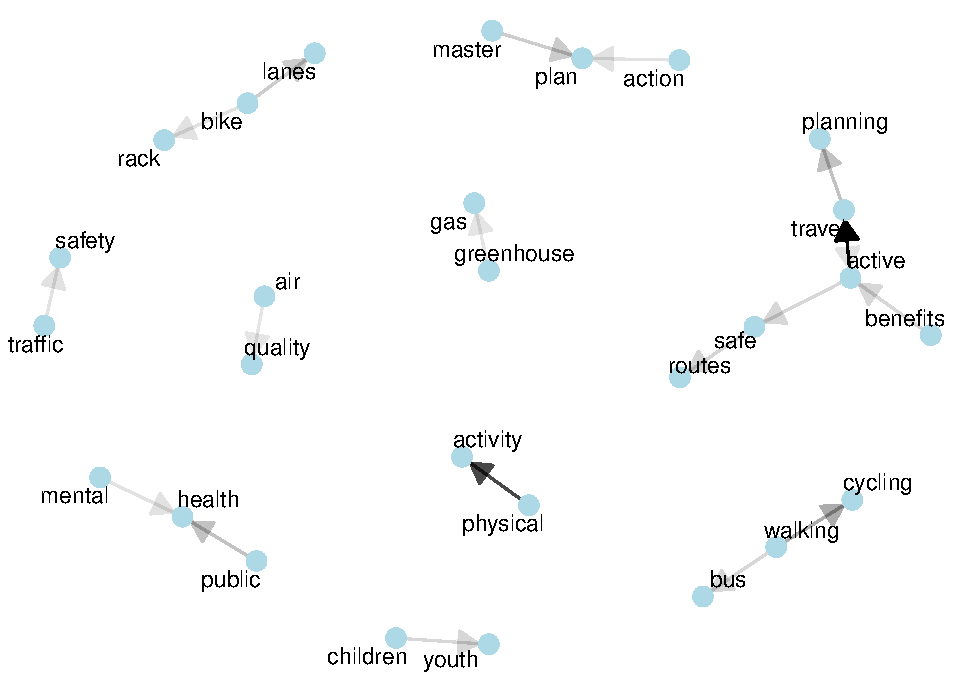
\includegraphics[width=1\linewidth]{AST-Framing-Ontario_files/figure-latex/city-visual-1} 

}

\caption{Most common bigrams found in the municipal or regional government documents.}\label{fig:city-visual}
\end{figure}

\begin{figure}

{\centering 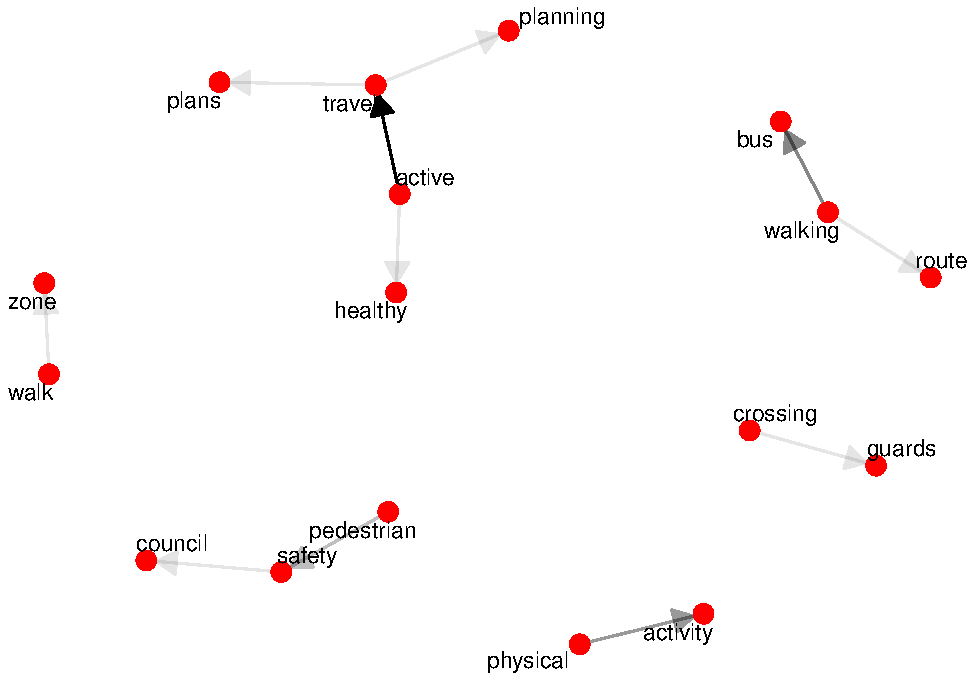
\includegraphics[width=1\linewidth]{AST-Framing-Ontario_files/figure-latex/consortia-visual-1} 

}

\caption{Most common bigrams found in the transportation consortia documents.}\label{fig:consortia-visual}
\end{figure}

\begin{figure}

{\centering 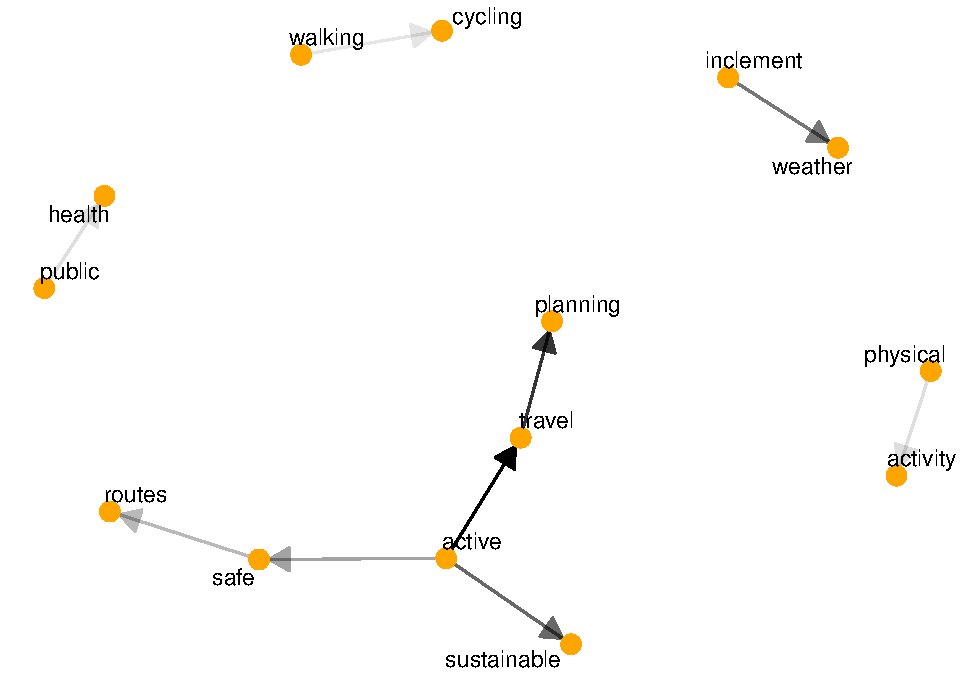
\includegraphics[width=1\linewidth]{AST-Framing-Ontario_files/figure-latex/school-visual-1} 

}

\caption{Most common bigrams found in the school board documents.}\label{fig:school-visual}
\end{figure}

\begin{figure}

{\centering 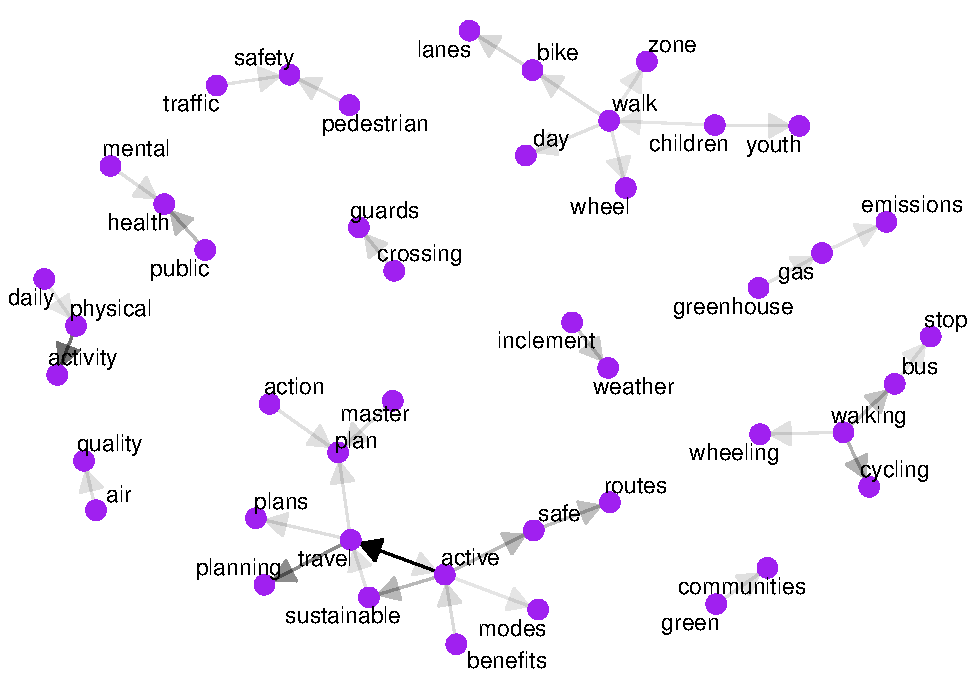
\includegraphics[width=1\linewidth]{AST-Framing-Ontario_files/figure-latex/policy-visual-1} 

}

\caption{Most common bigrams found in all of the policy documents (i.e., school board, municipality, and transportation consortia combined.}\label{fig:policy-visual}
\end{figure}

The academic corpora includes several common bigrams that were also
found in the policy documents including ``physical activity'' (n =
1566), which is the top bigram, ``traffic safety'' (n = 308), and ``safe
routes'' (n = 268). However, many other factors relating to AST are
identified in the research literature that are not presented to the
public through policy documents. After ``physical activity'', ``built
environment'' (n = 1175), ``independent mobility'' (n = 774), and
``urban form'' (n = 352) are the most frequent pairs of consecutive
words. Academic papers also often discuss ``distance home'' (n = 258),
``car ownership'' (n = 254), ``household income'' (n = 254), and
``population density'' (n = 205), which are factors that have been known
to influence AST. It is evident that many papers investigate gender
differences in AST given that ``boys girls'' (n = 211) is a common
bigram. Finally, the presence of ``statistically significant'' on the
list of top-25 bigrams underscores the importance of identifying factors
that are not due to chance but that likely influence AST.

\begin{figure}

{\centering 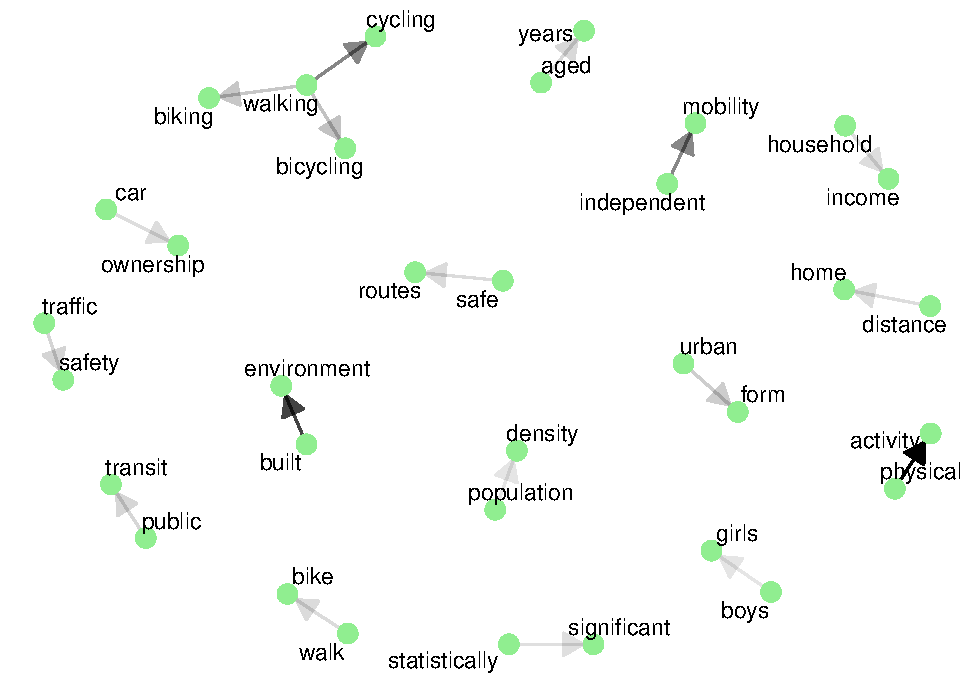
\includegraphics[width=1\linewidth]{AST-Framing-Ontario_files/figure-latex/academic-visual-1} 

}

\caption{Most common bigrams found in the academic papers.}\label{fig:academic-visual}
\end{figure}

\hypertarget{qualitative-findings-of-policy-documents}{%
\subsection{4.3. Qualitative findings of policy
documents}\label{qualitative-findings-of-policy-documents}}

We used the most common bigrams from the policy corpus (see Figure
\ref{fig:policy-visual}), which includes all documents from
municipalities, transportation consortia, and school boards, as
categories of codes for qualitative content analysis. This means that we
interpreted the bigrams to represent the main ideas that STP
stakeholders are communicating to the public about AST.

\hypertarget{discussion}{%
\section{5. Discussion}\label{discussion}}

\hypertarget{framing-of-ast-in-policy-documents}{%
\subsection{5.1. Framing of AST in policy
documents}\label{framing-of-ast-in-policy-documents}}

The presence of ``travel planning'' among the top pairs of consecutive
words for municipalities, school boards, and transportation consortia
reflects the

\hypertarget{framing-of-ast-in-academic-papers}{%
\subsection{5.2. Framing of AST in academic
papers}\label{framing-of-ast-in-academic-papers}}

Notably absent from the policy corpora is children's independent
mobility (CIM). AST is one of the most common opportunities for children
to travel without adult supervision on a regular basis, yet STP
stakeholders do not discuss this topic. CIM was first described by
Hillman et al.~({\textbf{???}}) as the freedom of children to travel and
play within their neighborhood and city without the presence of adults.
The ability of children to reach destinations such as school or local
parks by walking or bicycling on their own is a growing area of research
that is related to and often overlaps with the body of literature on
AST.

In a study conducted in multiple Canadian cities, Riazi et
al.~({\textbf{???}}) found that a range of factors such as child grade,
car ownership, and parental perceptions of safety and environment were
associated with CIM. Parental perceptions of children's autonomy also
influences CIM ({\textbf{???}}). In addition to independent trips to
school, children also travel by walking or bicycling on their own to
other non-school destinations such as outdoor spaces (i.e., parks,
playgrounds), the homes of family members or friends, shopping places,
and libraries, to name a few ({\textbf{???}}; {\textbf{???}}).

\hypertarget{implications-for-school-travel-planning}{%
\subsection{5.3. Implications for School Travel
Planning}\label{implications-for-school-travel-planning}}

School boards and educators are an influential contributor to AST and
STP efforts in Canada.

\hypertarget{limitations}{%
\subsection{5.4. Limitations}\label{limitations}}

\hypertarget{conclusion}{%
\section{6.1. Conclusion}\label{conclusion}}

\hypertarget{future-research}{%
\subsection{6.1. Future research}\label{future-research}}

\hypertarget{acknowledgments}{%
\section{Acknowledgments}\label{acknowledgments}}

This research was completed using open software, and the authors wish to
acknowledge the developers of the following \texttt{R} packages:
\texttt{dplyr} ({\textbf{???}}), \texttt{ggraph} ({\textbf{???}}),
\texttt{ggplot2} ({\textbf{???}}), \texttt{igraph} ({\textbf{???}}),
\texttt{pdftools} ({\textbf{???}}), \texttt{readr} ({\textbf{???}}),
\texttt{reshape2} ({\textbf{???}}), \texttt{stringr} ({\textbf{???}}),
\texttt{text2vec} ({\textbf{???}}), \texttt{textdata} ({\textbf{???}}),
\texttt{tidyr} ({\textbf{???}}), \texttt{tidytext} ({\textbf{???}}),
\texttt{tm} ({\textbf{???}}), \texttt{tools} ({\textbf{???}}),
\texttt{topicmodels} ({\textbf{???}}), \texttt{widyr} ({\textbf{???}}),
\texttt{word2vec} ({\textbf{???}}), \texttt{wordcloud} ({\textbf{???}}),
\texttt{DiagrammeR} ({\textbf{???}}), and \texttt{kableextra}
({\textbf{???}}).

\hypertarget{references}{%
\section{References}\label{references}}


\end{document}


